\subsection{Spektroskopi}

Spektroskopi benytter seg av fotoluminisens. N�r et elektronhullpar rekombinerer sendes energien som blir frigitt ut som et foton. Ved � m�le energien til fotonet kommer det fram hvor mye energi som ble frigitt under rekombinering. Dette sier noe om b�ndgapet til materialet, som igjen er en beskrivelse av hva slags materiale det er. Ved � belyse en pr�ve med lys som har h�y energi og intensitet, vil det eksiteres lys til alle tilgjengelige tilstander. N�r disse tilstandene rekombinerer vil det sendes lys ut av pr�ven som kan fanges opp av et kamera og analyseres av en datamaskin for � f� ut et spekter av ulike b�lgelengder. For enkrystallinsk silisium er b�ndgapet 1.1eV, som f�rer til h�y intensitet av lys med 1.1eV energi.

\begin{figure}%
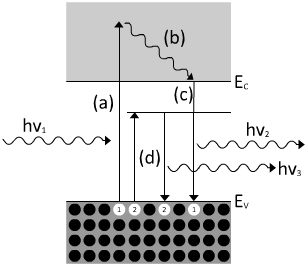
\includegraphics[width=10cm,bb=0 0 306 265]{luminisence.png}%
\caption{Eksitasjon og rekombinering}%
\label{fig:luminisens}%
\end{figure}

Figur \ref{fig:luminisens} viser inkommende lys med h�y energi som eksiterer et elektron hullpar i $a$, som etter meget kort tid faller ned til en lavere energitilstand i $b$. I $c$ rekombinerer elektronet og det sendes ut et foton med energi lik $E_c$. Det andre elektronet som eksiteres i $d$ havner i en s�kalt "`trap"' state, hvor det kan befinne seg forurensninger eller defekter i en krystallstruktur. N�r dette elektronet rekombinerer sendes det ut et foton med lavere energi enn i $c$. Ved � se p� lyset som kommer ut fra en slik trap state kan det lokaliseres blant annet forurensninger. 